\documentclass[11pt, a4paper]{article}
\usepackage[english]{babel}
\usepackage[utf8]{inputenc} 
\usepackage[T1]{fontenc}
\usepackage{bm}
\usepackage{graphicx}
\usepackage{multirow}
\usepackage[table,xcdraw]{xcolor}
\usepackage{hhline}
\usepackage{comment}
\usepackage{amsmath, amsfonts, latexsym, color, textcomp, anysize}
\usepackage[rightcaption]{sidecap}
\usepackage{url}
\usepackage{tablefootnote}
\usepackage{fancyhdr}
\usepackage{blindtext}
\usepackage{scrextend}
\addtokomafont{labelinglabel}{\sffamily}
\usepackage{caption}% descomentar de querer texto mais pequeno nas captions de figura e taboas
\captionsetup{font = footnotesize} % descomentar de querer texto mais pequeno nas captions de figura e taboas. Existen mais opcions en internet.
\usepackage{subfigure}
\marginsize{3cm}{3cm}{3cm}{3cm}
\setlength{\headheight}{13.59999pt}
\parindent=2mm %sangría
\parskip=2.5mm   %separacion entre parrafos
\usepackage{gensymb}
\usepackage{wrapfig}
%\usepackage{natbib}
\usepackage[hidelinks, pdftex]{hyperref}

\definecolor{unipd}{RGB}{162, 0, 23}
\definecolor{white-grey-ish}{RGB}{234, 236, 240}
\newcommand{\abs}[1]{\lvert#1\rvert}

%%%%%%%%%%%%%%%%%%%%%%%%%%%%%%%%%%
%%%%%%%%%%%% ata aquí a plantilla %%%%%%%%%%%%
%%%%%%%%%%%%%%%%%%%%%%%%%%%%%%%%%%

\usepackage{enumerate}
\usepackage{float}
\usepackage{booktabs}

\newcommand{\TeV}{\textrm{ }\mathrm{TeV}}
\newcommand{\GeV}{\textrm{ }\mathrm{GeV}}
\renewcommand{\H}{{\rm H}}
\newcommand{\Z}{{\rm Z}}
\newcommand{\JPsi}{{\rm J}/\psi}
\newcommand{\pt}{p_{\rm T}}
 
\bibliographystyle{elsarticle-num}


\begin{document}

\pagenumbering{Roman}
\pagestyle{empty}

% front page
\begin{center}
\vspace{3em}

\includegraphics[width=25em]{images/logo_800anni.png}\\
\vspace{3em}
\begin{tabular}[c]{c}
{\large\color{unipd} \sc Dipartimento di Fisica e Astronomia} \vspace{0.5em}\\
{\large\color{unipd} \sc MSc in Physics} \vspace{2.7em}\mbox{}
\end{tabular}

\vspace{2cm}
\rule{65mm}{0.2mm}\\
\vspace{1cm}

{\sc\LARGE Research Activities report}\\$\ $\\
{\sl\large  Analysis of the current trigger and selection efficiency}\\ 
{\sl\large  for the process $\H \rightarrow \JPsi\gamma \rightarrow \mu\mu\gamma$ at CMS}\\
{\sl\large  and comparison with new trigger proposals}

\vspace{0.5cm}
\rule{65mm}{0.2mm}\\
\vspace{2cm}
\end{center}

\vspace{\fill}
\begin{tabular}{l}
{\sl\large Author:} \\
{\bf\Large Javier Mariño Villadamigo}
\vspace{1em}\mbox{} \\

{\sl\large Supervisor:} \\
{\bf\large Alberto Zucchetta} \\
{\sl\large Area FIS/01-FIS/04}\\
{\sl\large Department of Physics}
\vspace{1em}\mbox{} \\
\end{tabular}

\begin{center}
\vspace{\fill}
{\Large\color{unipd} October 2022}
\end{center}

%%%%%%%%

% blank page with roman numbering after front 
\clearpage
$\ $
\pagestyle{fancy}
\fancypagestyle{plain}
\lhead{}
\chead{}
\rhead{}
\renewcommand{\headrulewidth}{0pt}
\lfoot{} 
\cfoot{\thepage}
\rfoot{} 
\renewcommand{\footrulewidth}{0pt}

%%%%%%%%
% uncomment for blank intermediate pages %
\begin{comment}
% abstract page
\newpage
\clearpage
\begin{abstract}
The abstract goes here.
\end{abstract}

%%%%%%%%

% blank page with roman numbering after abstract 
\clearpage
$\ $
\pagestyle{fancy}
\fancypagestyle{plain}
\lhead{}
\chead{}
\rhead{}
\renewcommand{\headrulewidth}{0pt}
\lfoot{} 
\cfoot{\thepage}
\rfoot{} 
\renewcommand{\footrulewidth}{0pt}

% contents page
\clearpage
\pagestyle{fancy}
\fancypagestyle{plain}
\lhead{}
\chead{}
\rhead{}
\renewcommand{\headrulewidth}{0.1pt}
\lfoot{} 
\cfoot{\thepage}
\rfoot{} 
\renewcommand{\footrulewidth}{0pt}
\tableofcontents

%%%%%%%%

% blank page with roman numbering after contents 
\clearpage
$\ $
\pagestyle{plain}
\fancypagestyle{empty}
\lhead{}
\chead{}
\rhead{}
\renewcommand{\headrulewidth}{0pt}
\lfoot{} 
\cfoot{\thepage}
\rfoot{} 
\renewcommand{\footrulewidth}{0pt}
\end{comment}
%%%%%%%%


% abstract page
\begin{abstract}
This work is presented as the final report of the research activities carried out for the correspondent course ({\it Introduction to research} with code SCQ1097888) held at the Department of Physics, University of Padua. The main activities were developed during the month of September of the year 2022. These were focused on the analysis of the efficiency of a specific trigger, used for the identification of signal events coming from the exotic Higgs boson decay $\H \rightarrow \JPsi\gamma \rightarrow \mu\mu\gamma$ at CMS. A comparison between the selection efficiency related to the standard trigger and other types of selections has been made. As a result, it has been found that other triggers, which attend to not only purely kinematical criteria, may be more suitable for the studies of the aforementioned decay.
\end{abstract}

%%%%%%%%

% contents page
\clearpage
\pagestyle{fancy}
\fancypagestyle{plain}
\lhead{}
\chead{}
\rhead{}
\renewcommand{\headrulewidth}{0.1pt}
\lfoot{} 
\cfoot{\thepage}
\rfoot{} 
\renewcommand{\footrulewidth}{0pt}
\tableofcontents

% start of report
\clearpage
\pagenumbering{arabic}\setcounter{page}{1}
\section{Introduction\label{sec:introduction}}
The Higgs boson is considered to be discovered in 2012, when a boson of 125 GeV of mass, compatible with the Higgs boson, was discovered by CMS \cite{commissioningCMS} and ATLAS \cite{commissioningATLAS} collaborations. Many properties of such boson have been so far analyzed, but its Yukawa couplings to first and second generation quarks are still to be measured.

In this vein, rare exclusive decays of the Higgs boson to mesons in association with a photon can be used to explore such couplings. In particular, the decay $\H \rightarrow \JPsi\gamma$ (being $\JPsi$ a bound paired state of charm quark-antiquark) can be used to test the coupling of the Higgs boson to the charm quark. 
The corresponding decay $\Z \rightarrow \JPsi\gamma$ is normally used as an experimental benchmark in the search for the Higgs exotic decay. Both decays receive contributions from direct and indirect processes, which are detailed in Fig. \ref{im:direct_and_indirect_processes}.

\begin{figure}[htbp]
    \centering
    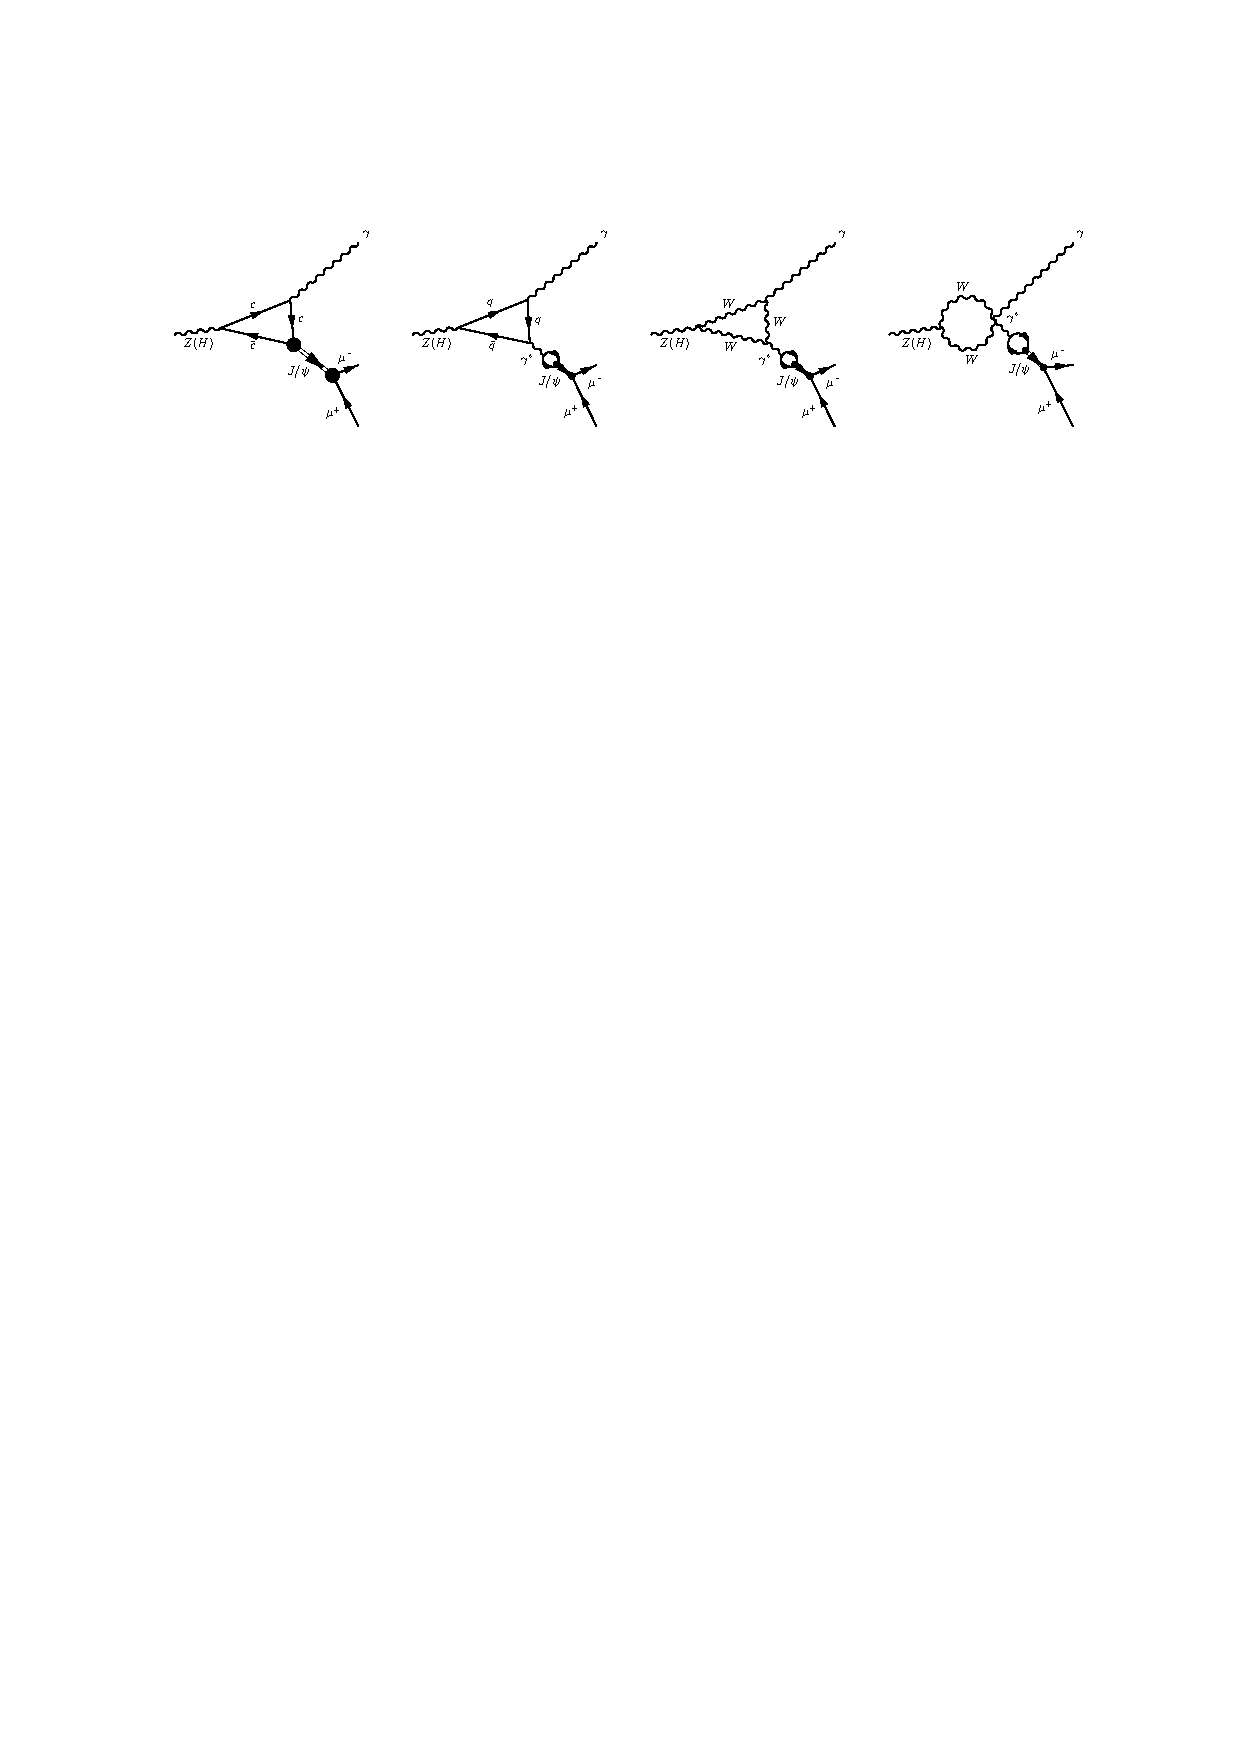
\includegraphics[width=0.9\linewidth]{images/direct_and_indirect_processes.pdf}
    \caption{From \cite{mainarticle}: lowest order Feynman diagrams for the $\Z$ (or $\H$) $\rightarrow \JPsi\gamma$ decay. The left-most diagram shows the direct and the remaining diagrams the indirect processes.
    \label{im:direct_and_indirect_processes}}
\end{figure}

Since the yield produced from the Higgs boson decay is proportional to the ${\rm Hc\bar{c}}$ coupling, measurements of the branching ratio (BR) of such decay could provide information on whether this coupling deviates from the Standard Model (SM) prediction. As an example, if the ${\rm Hc\bar{c}}$ coupling deviates by more than a factor 2 from the SM value, the shift in the BR for $\H \rightarrow \JPsi\gamma$ can be more than 100\% \cite{PhysRevD.88.053003}.

So far, however, the experimental efforts to determine this BR have only been able to establish an upper bound to the value, which is of the order of 200 times the SM prediction \cite{mainarticle}. One of the main challenges this particular search is facing is the discrimination between signal events and background. To tackle this matter, more integrated luminosity to enhance the discrimination between the Z and Higgs signals and the background and, if feasible, a more efficient trigger, are needed.

\section{Objectives}
The LHC can reach up to 40 million bunches of protons crossing the detector zone every second, and it is not possible to record every single collision, so the amount of initial information has to be filtered in some way. This filtering does not only need to be efficient, recording as many events of interest as possible (while dismissing those that are not), but it also needs to be quick.

To achieve this, CMS bears a two-level trigger. In the case of study, the lowest level L1 keeps the event if it contains a detected muon with $\pt$ greater than $5 \GeV$ and an isolated electromagnetic object with $\pt$ greater than $18\GeV$, giving rise to a rate of events fulfilling L1 conditions of around $100\textrm{ }\mathrm{kHz}$ . The second-level, or High Level Trigger (HLT), on the other hand, requires the presence of a muon and a photon exceeding 17 and 30 $\GeV$, respectively, reducing the rate of 100 kHz fulfilling L1 to around 1 kHz fulfilling HLT, which is finally written to disk. This HLT is conveniently called {\it HLT\_Mu17\_Photon30}.

The goal of this study is therefore to re-design a new possible trigger that can improve the performance of the {\it HLT\_Mu17\_Photon30} currently in use. A new trigger would be better than the current one if it could provide a higher efficiency for the acquisition of signal events and/or reduce the amount of background that it records.

\section{Trigger and selection efficiencies}
In order to quantify the efficiency of a trigger and design a new possible one, two quantities have to be introduced. The first one is the {\bf trigger efficiency}, which is defined as the ratio of the events that satisfy the selection of interest AND also pass the trigger, divided by the events that satisfy the selection of interest:
\begin{equation}
    \varepsilon_{\rm trigger} = \frac{{\rm \#\ events\ passing\ HLT\ \& \ selection}}{{\rm \#\ events\ passing\ selection}}
    \label{eq:trigger_efficiency}
\end{equation}
On the other hand, the {\bf selection of interest}, which will also be called selection criteria, or simply selection, is the name given to a set of conditions the events have to fulfill in order to be considered. For example, for the study of the decays of interest of the Z and the Higgs boson, the standard selections are listed in Table \ref{tab:selection}.
 
\begin{table}[htbp]
	\centering
	\begin{tabular}{cc}
		\toprule
		\multicolumn{1}{c}{{\bf Muons}} & \multicolumn{1}{c}{{\bf Photons}} \\ \midrule
		${\rm nMuon} \geq 2$ & ${\rm nPhoton} \geq 1$ \\
		Opposite charges: $\mu^{-},\ \mu^{+}$ & - \\
		$|\eta| < 2.4$ & $|\eta| < 2.4$\\
		Retain pair with min. $\Delta R = \sqrt{(\Delta\phi)^{2}+(\Delta \eta)^{2}}$ & - \\
        $\pt^{\mu_{1}}> 10\GeV,\ \pt^{\mu_{2}} > 5\GeV$ & $\pt^{\gamma} > 15 \GeV$ \\
        mediumId & mvaID\_WP90 \\
       - & pixel\_Seed $=$ 0 \\
        \bottomrule
	\end{tabular}
	\caption{Kinematic, charge and quality selection criteria imposed to the muons and photons in the final state.}
	\label{tab:selection}
\end{table}

The first filter of events regarding the muons is their number in the final state: at least two are required to be present. The leading and subleading muon should have a transverse momentum $\pt > 10\GeV$ and $\pt > 5\GeV$, respectively, and carry opposite charges. Then, only the pair with the smallest angular separation $\Delta R$ is retained, as this is the one likely produced from the decay of the $\JPsi$. The next requirement is ``mediumId'', which is demanded to be true for both muons, and refers to the quality of the identification of muons. A loose identification is highly efficient, but increases the probability of misidentification. A tight identification is less efficient, but has a lower probability of misidentification. Here, a medium criterion was used, which is a compromise between loose and tight.

Photons, on the other hand, are required to be present in the final state with at least one of momentum threshold of $\pt > 15 \GeV$. The photon must also satisfy a multivariate discriminant called ``mvaID\_WP90'', which refers to the efficiency of the identification; a closer value to 100 signifies a higher efficiency in the identification. Finally, ``pixel\_Seed'' is required to be 0 (or simply ``false''), which is the same as requiring the photon to not leave track in the silicon detector pixels.

For both muons and photons, the pseudo-rapidity $\eta$ is required to have an absolute value smaller than 2.4, which is a criterion regarding the transversality of the emitted photon and muons with respect to the beam axis. Since $\eta \equiv -\log (\tan\theta / 2)$, being $\theta$ the angle with respect to the beam axis, a value $\eta = 0$ ($\theta = \pi/2$) corresponds to a particle detected transversely, while $\eta\rightarrow \pm\infty$ ($\theta = 0,\ \pi$) corresponds to a particle emitted parallel/antiparallel to the beam axis.

These selections, summarized in Table \ref{tab:selection}, will be common for the rest of the analysis, so they must be understood as base selections, {\it inherent} to the analyzed data. In some cases, nevertheless, some of the kinematical criteria will be more strict. For example, when the transverse momentum thresholds are imposed to be higher (never lower), it will be correspondingly specified.

Since the trigger is a piece of software dedicated to the selection of events, it is not possible to compute directly the efficiency of a newly proposed one. Instead, one has to run dedicated simulations to do so. In this work, the corresponding selection efficiency has been used instead. The {\bf selection efficiency} is defined as the number of events that pass a set of selection criteria, divided by the total number of events in the data set:
\begin{equation}
    \varepsilon_{\rm selection} = \frac{{\rm \#\ events\ passing\ selection}}{{\rm \#\ total\ events}}
    \label{eq:selection_efficiency}
\end{equation}
This selection efficiency closely resembles, for the signal events, the trigger efficiency. The eventual discrepancies between both, usually of the order of a few percent, are related to the difference in the offline and online reconstruction algorithms.

It is important to note that both the numerator and the denominator in Eq. \ref{eq:selection_efficiency} refer to events from the same category, i.e. the efficiency of selection for the Higgs boson signal will be computed as the total number of Higgs events passing the corresponding selection, divided by the total number of Higgs events.

\subsection{The uncertainty of the efficiency}
An efficiency is, as it has just been defined, calculated as the fraction between the number of certain accepted events, over the total number of events in a sample. The number of events in a given sample, or the number of selected events, both follow a Poisson distribution, and have thus an uncertainty given by $\sigma(N) = \sqrt{N}$. Since the application of a cut can be considered a binomial process (an event either does or does not pass a certain selection), the uncertainty for the efficiency can be calculated \cite{paterno2004calculating} as:
\begin{equation}
    \sigma(\varepsilon) = \frac{1}{N}\sqrt{k\left (1-\frac{k}{N}\right )},
    \label{eq:uncertainty_eff}
\end{equation}
where $N$ is the total number of events in the sample on which the efficiency is calculated and $k$ is the number of events that pass the cut i.e. $\varepsilon = k/N$. It is important to note that this type of calculation fails when the number of events accepted is either 0 or $N$, but since this problem will not be encountered in this work, and improving the calculation requires a large increase in complexity, Eq. \ref{eq:uncertainty_eff} is the one that will be used to compute the uncertainties for the efficiencies calculated.

\section{Data samples}
In order to compute the efficiency of a selection, it is required to have previous knowledge on the nature of the dataset. Consequently, the data samples used for this work were 3 simulated samples of QCD background, Z signal and Higgs signal, respectively, all generated with the software {\sc pythia 8} \cite{pythia}. The QCD sample has been generated with a muon-enriched final state in order to have a reasonable number of events passing the selections. All the Z and Higgs boson data samples have been generated to decay in the $\JPsi\gamma\rightarrow \mu\mu\gamma$ process. The total number of events in each data sample is detailed in Table \ref{tab:events_generated}.

% Table generated by Excel2LaTeX from sheet 'Sheet1'
\begin{table}[htbp]
    \centering
        \begin{tabular}{ccc}
        \toprule
        \multicolumn{3}{c}{Total number of events generated} \\ \midrule
        QCD   & Z     & H \\
        $(21336\pm5)\cdot 10^{3}$ & $(4590\pm7)\cdot 10^{2}$ & $(4480\pm7)\cdot 10^{2}$ \\ \bottomrule
        \end{tabular}%
        \caption{Total number of events generated for QCD background, Z and Higgs signals samples.
    \label{tab:events_generated}}
\end{table}%

For a given set of selection criteria, the same cuts will be applied to all the three types of data sets, and the corresponding selection efficiencies will be compared with those of the {\it HLT\_Mu17\_Photon30}.

\subsection{The selection efficiency for {\it HLT\_Mu17\_Photon30}}
Even though it has not been mentioned up to now, the use of {\it HLT\_Mu17\_Photon30} trigger has a further selection criteria apart from the ones showed in Table \ref{tab:selection}. The selected events, in this case, are furthermore required to have a muon with $\pt > 18\GeV$, whereas the cut in the photon momentum is increased to $\pt > 32\GeV$.

Given the fact that this is the first example, a detailed calculation of the trigger and selection efficiencies will be shown, but for the new selections studied in the following sections and for the sake of clarity, only the final result will be displayed.

% Table generated by Excel2LaTeX from sheet 'Sheet1'
\begin{table}[htbp]
  \centering
    \resizebox{\textwidth}{!}{
    \begin{tabular}{c|ccc|cc} \toprule
          & \multicolumn{5}{c}{\it HLT\_Mu17\_Photon30} \\ \midrule
          & & & & \multicolumn{2}{c}{Efficiencies (\%)} \\
          & {\rm \# total events} & {\rm \#  passing sel.} & {\rm \#  passing HLT \& sel.} & {\bf Trigger} & {\bf Selection} \\ \midrule
    QCD   & $(21336\pm5)\cdot 10^{3}$ & $34\pm6$    & $26\pm5$    & $76\pm7$ & $(1.6\pm 0.3)\cdot 10^{-4}$ \\
    Z     & $(4590\pm7)\cdot 10^{2}$ & $(986\pm3)\cdot 10 ^{2}$ & $(818\pm3)\cdot 10 ^{2}$ & $83.0\pm 0.1$ & $21.49\pm0.06$ \\
    H     & $(4480\pm7)\cdot 10^{2}$ & $(1606\pm4)\cdot 10 ^{2}$ & $(1421\pm4)\cdot 10 ^{2}$ & $88.49\pm 0.08$ & $35.85\pm 0.07$ \\ \bottomrule
    \end{tabular}}
      \caption{Example calculation of the trigger and selection efficiencies for the trigger {\it HLT\_Mu17\_Photon30} and selection cuts: $\pt^{\mu}>18\GeV$ and $\pt^{\gamma}>32\GeV$.
  \label{tab:addlabel}}
\end{table}%

As described in Eqs. \ref{eq:trigger_efficiency} and \ref{eq:selection_efficiency}, the trigger efficiency has been obtained dividing the third column by the second one, and the selection efficiency, on the other hand, dividing the second column by the total number of events in the first column.

As expected, the selection efficiency for QCD events is substantially lower than for the signal samples, since the selection criteria have been specifically tailored for the latter. However, its trigger efficiency (around 76\%) is comparable to those of Z and Higgs (around 85\%). This means that once an event of background has passed the selection criteria, the probability of it passing the High Level Trigger is comparable to the one that signal events have. The ``trick'' in these studies is that the selection cuts must reduce to the maximum the number of undesired events (hence reducing also the undesired events that pass the HLT) while maintaining a reasonable efficiency in signal acceptance.

\section{Results}
In this section, the results for selection efficiency, using 5 different selection criteria, are presented. These will be compared to the ones obtained for {\it HLT\_Mu17\_Photon30} (keeping in mind that the latter uses the $\pt^{\mu}>18\GeV$, $\pt^{\gamma}>32\GeV$ selection cuts). At the end of the section, a comprehensive figure is shown to display the 5 different possibilities studied along with the original trigger. In the following, the leading muon (i.e. the one with higher momenta) will be named muon1, whereas the subleading one will be muon2.

\subsection{Muon1: $\pt > 15\GeV$, muon2: $\pt > 10\GeV$, photon: $\pt>15\GeV$\label{sec:Mu15_Mu10_Photon15}}
The first attempt to increase Z and H acceptance and decrease that of QCD, has been softening the cuts on the muon1 and the photon, and to add an extra cut for the muon2. The results are shown in Table \ref{tab:Mu15_Mu10_Photon15}.

% Table generated by Excel2LaTeX from sheet 'Tables to present'
\begin{table}[htbp]
  \centering
    \resizebox{\textwidth}{!}{
    \begin{tabular}{ccc}
        \toprule
        & \multicolumn{2}{|c}{Selection efficiencies (\%)} \\ \midrule
        & \multicolumn{1}{|c|}{$\pt^{\mu 1} > 18\GeV$, $\pt^{\gamma} > 32\GeV$} & $\pt^{\mu 1} > 15\GeV$, $\pt^{\mu 2} > 10\GeV$, $\pt^{\gamma} > 15\GeV$ \\ \midrule
        QCD   & \multicolumn{1}{|c|}{$(1.6\pm 0.3)\cdot 10^{-4}$} & $(4.4\pm0.5)\cdot 10 ^{-4}$ \\
        Z     & \multicolumn{1}{|c|}{$21.49\pm0.06$} &  $20.55\pm0.06$ \\
        H     & \multicolumn{1}{|c|}{$35.85\pm 0.07$} &  $28.65\pm0.07$ \\ \bottomrule
    \end{tabular}}
    \caption{Selection efficiencies obtained for the selection cuts: $\pt^{\mu 1} > 15\GeV$, $\pt^{\mu 2} > 10\GeV$, $\pt^{\gamma} > 15\GeV$ (right column) compared to the ones obtained for $\pt^{\mu 1} > 18\GeV$, $\pt^{\gamma} > 32\GeV$ (left column).
    \label{tab:Mu15_Mu10_Photon15}}
\end{table}%

As it can be seen, the efficiencies have decreased for both Z and Higgs signals, while increasing for the QCD background, thus worsening the initial results. After only a few tests, the conclusion is that the selection efficiency for Z and Higgs signals can only be recovered for an increased QCD efficiency, and so this scheme for the selection cuts is discarded.

\subsection{Muon1: $\pt > 18\GeV$, photon: $\pt>24\GeV$, $\Delta R(\mu-\mu)<0.4$ \label{sec:Mu18_Ph24_dR04}}
As stated in Section \ref{sec:introduction}, the two muons in the final state proceed from the decay of the $\JPsi$ meson, rather than from in-flight decays of hadrons (or other processes) in the case of background. Therefore, both muons are expected to be highly collinear or, in other words, have small angular separation. This angular separation between the two muons for QCD, Z and Higgs events is shown in Fig. \ref{im:dR_mumu_combined}.

\begin{figure}[htbp]
    \centering
    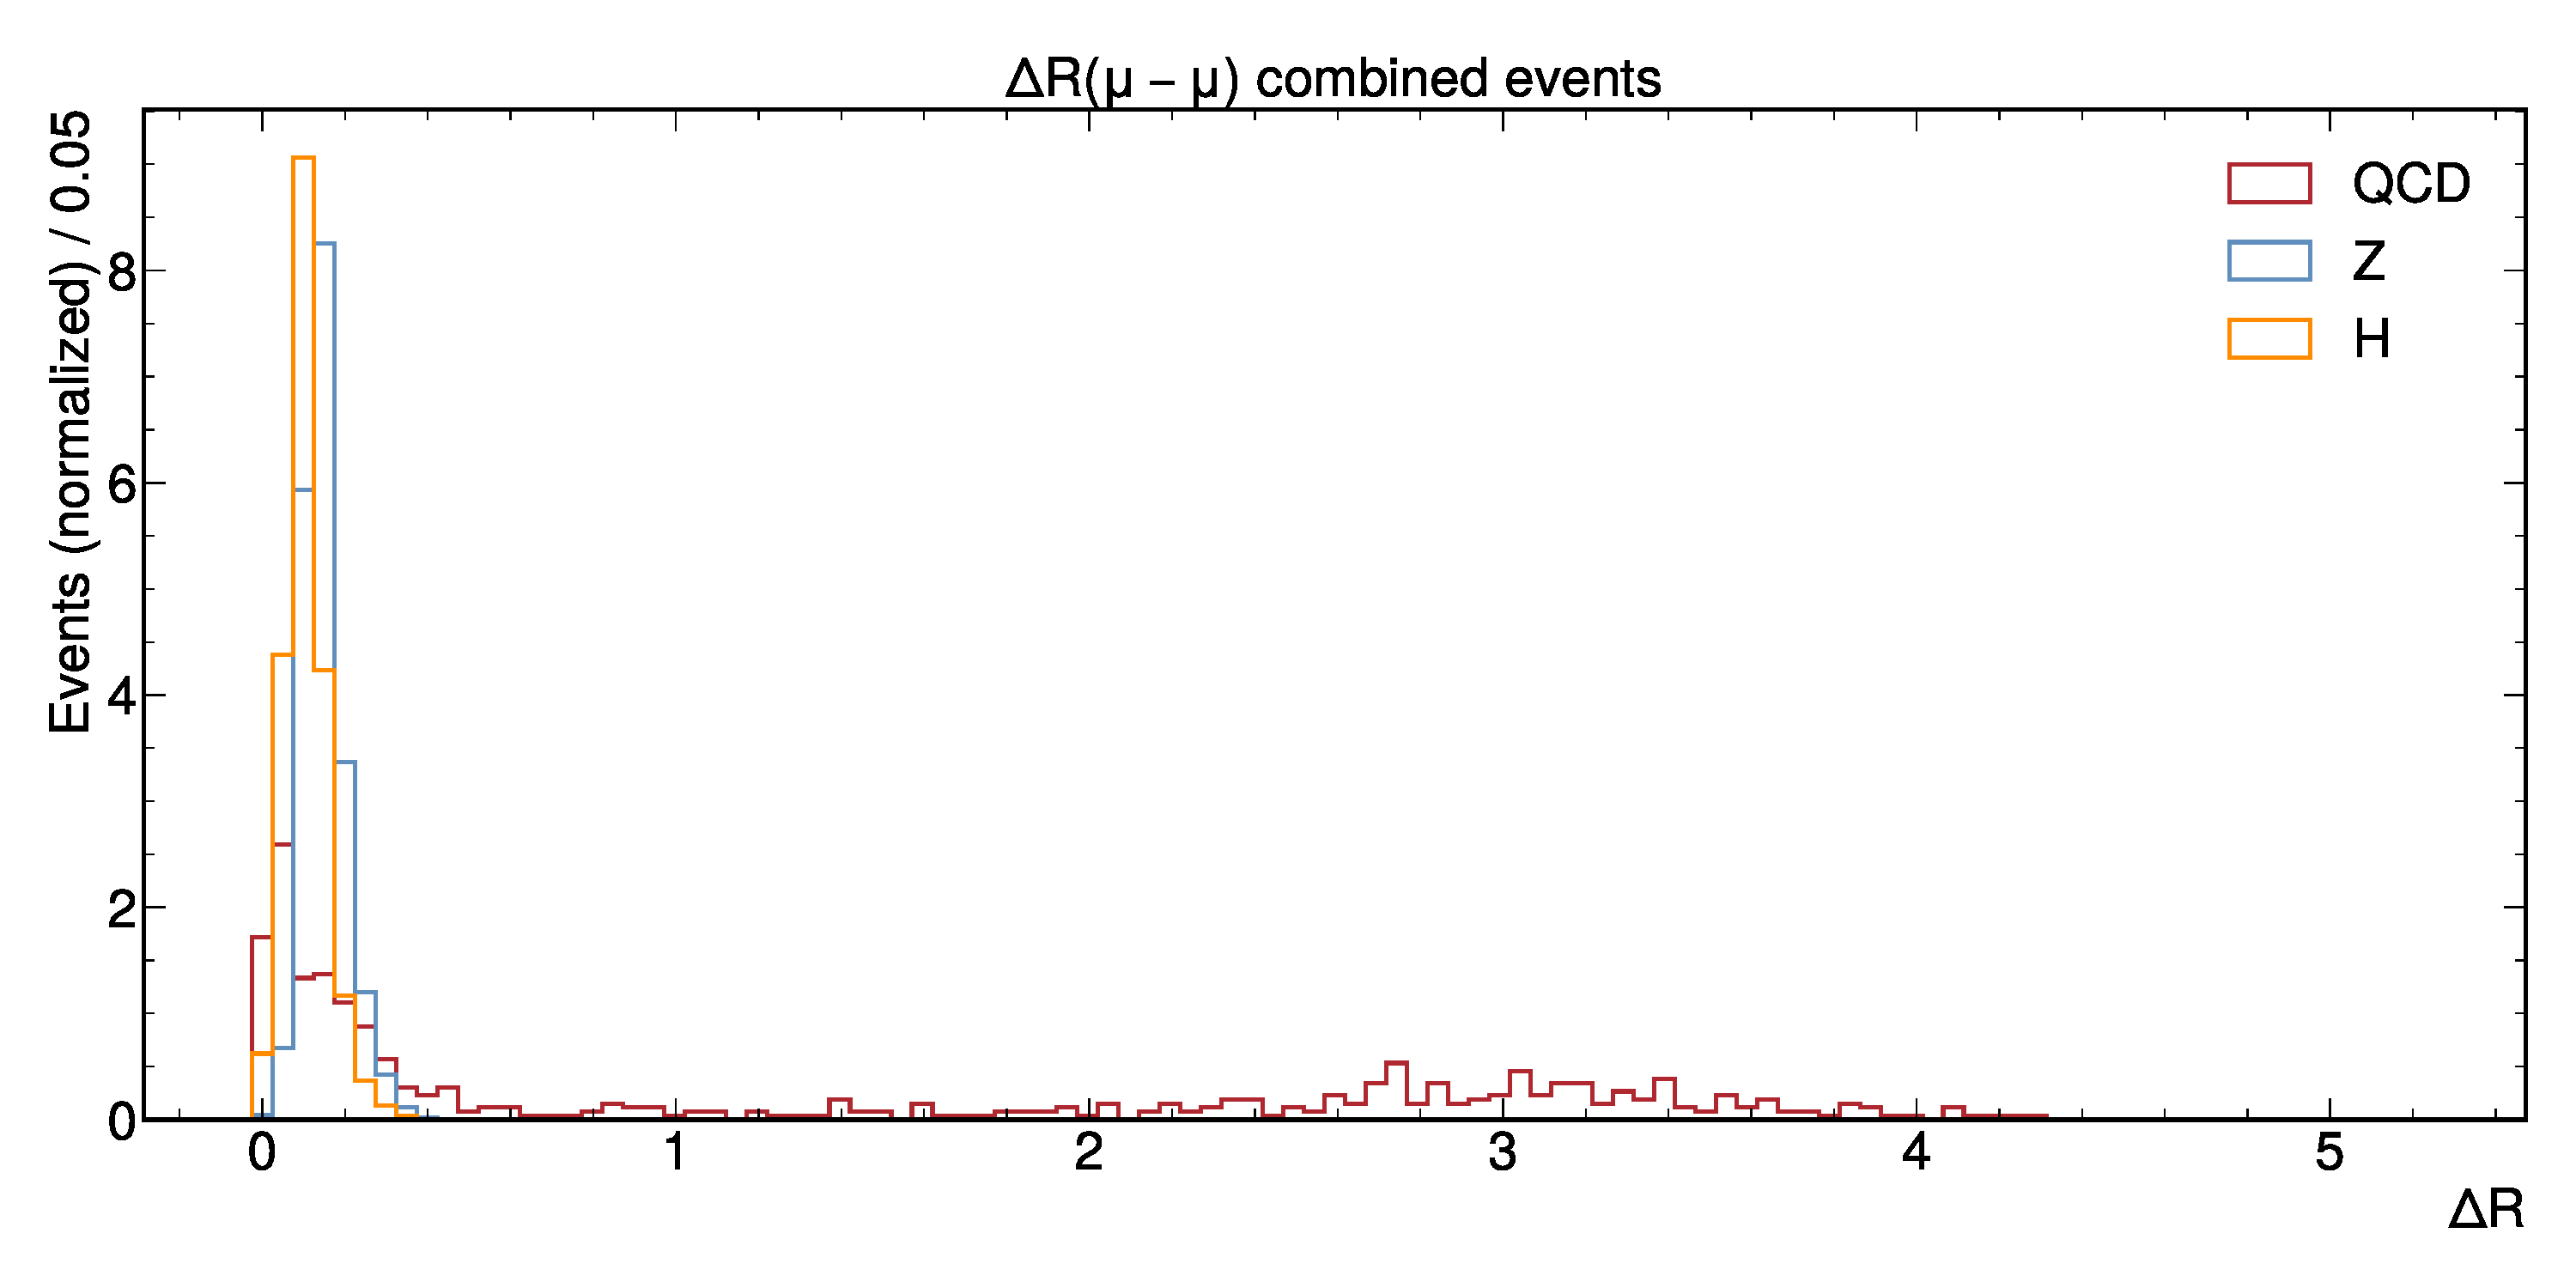
\includegraphics[width=.9\linewidth]{images/dR_mumu_combined.pdf}
    \caption{Angular separation $\Delta R$ between the two muons reconstructed in the final state. Base selection criteria from Table \ref{tab:selection} have been applied in order to observe the distribution in $\Delta R$. The number of events in each histogram has been normalized so that the integral is equal to 1.
    \label{im:dR_mumu_combined}}
\end{figure}

Indeed, the angular separation $\Delta R$ is rather uniformly distributed for QCD events, between 0 and almost $2\pi$. Z and Higgs signals, however, show a clear accumulation for very small $\Delta R$, indicating that the muons are indeed emitted with high collinearity.

With this in mind, an upper bound of $\Delta R<0.4$ has been imposed for the second selection scheme, and the optimal values for the muon1 and photon momenta thresholds have been found to be 18 GeV and 24 GeV, respectively. The selection efficiencies obtained for this set of selections are shown in Table \ref{tab:Mu18Mu24dR04}.

% Table generated by Excel2LaTeX from sheet 'Tables to present'
\begin{table}[htbp]
  \centering
    \resizebox{\textwidth}{!}{
    \begin{tabular}{ccc}
        \toprule
        & \multicolumn{2}{|c}{Selection efficiencies (\%)} \\ \midrule
        & \multicolumn{1}{|c|}{$\pt^{\mu 1} > 18\GeV$, $\pt^{\gamma} > 32\GeV$} & $\pt^{\mu 1} > 18\GeV$, $\pt^{\gamma} > 24\GeV$, $\Delta R(\mu-\mu) <0.4$ \\ \midrule
        QCD   & \multicolumn{1}{|c|}{$(1.6\pm 0.3)\cdot 10^{-4}$} & $(1.4\pm0.3)\cdot 10^{-4}$ \\
        Z     & \multicolumn{1}{|c|}{$21.49\pm0.06$} &  $24.73\pm0.06$ \\
        H     & \multicolumn{1}{|c|}{$35.85\pm 0.07$} &  $37.65\pm0.07$ \\ \bottomrule
    \end{tabular}}
    \caption{Selection efficiencies obtained for the selection cuts: $\pt^{\mu 1} > 18\GeV$, $\pt^{\gamma} > 24\GeV$, $\Delta R(\mu-\mu) <0.4$ (right column) compared to the ones obtained for $\pt^{\mu 1} > 18\GeV$, $\pt^{\gamma} > 32\GeV$ (left column).
    \label{tab:Mu18Mu24dR04}}
\end{table}%

As a result, this selection scheme decreases the QCD efficiency by around a 10\%, while increasing the efficiency for Z signal around 15\%, and for Higgs signal around 5\%. These results are already better than those obtained for the current HLT, but they may still be improved.


\subsection{Muon1: $\pt > 15\GeV$, photon: $\pt>20\GeV$, $2\GeV<m_{\mu\mu}<4\GeV$}
Another characteristic feature of the muon pair, besides its expected small angular separation, is that, since they proceed from the decay of the $\JPsi$, their invariant mass should be that of the meson, which is 3.1 GeV. The invariant mass of the muon pair is shown in Fig. \ref{im:m_mumu_combined_TestForCut}.

\begin{figure}[htbp]
    \centering
    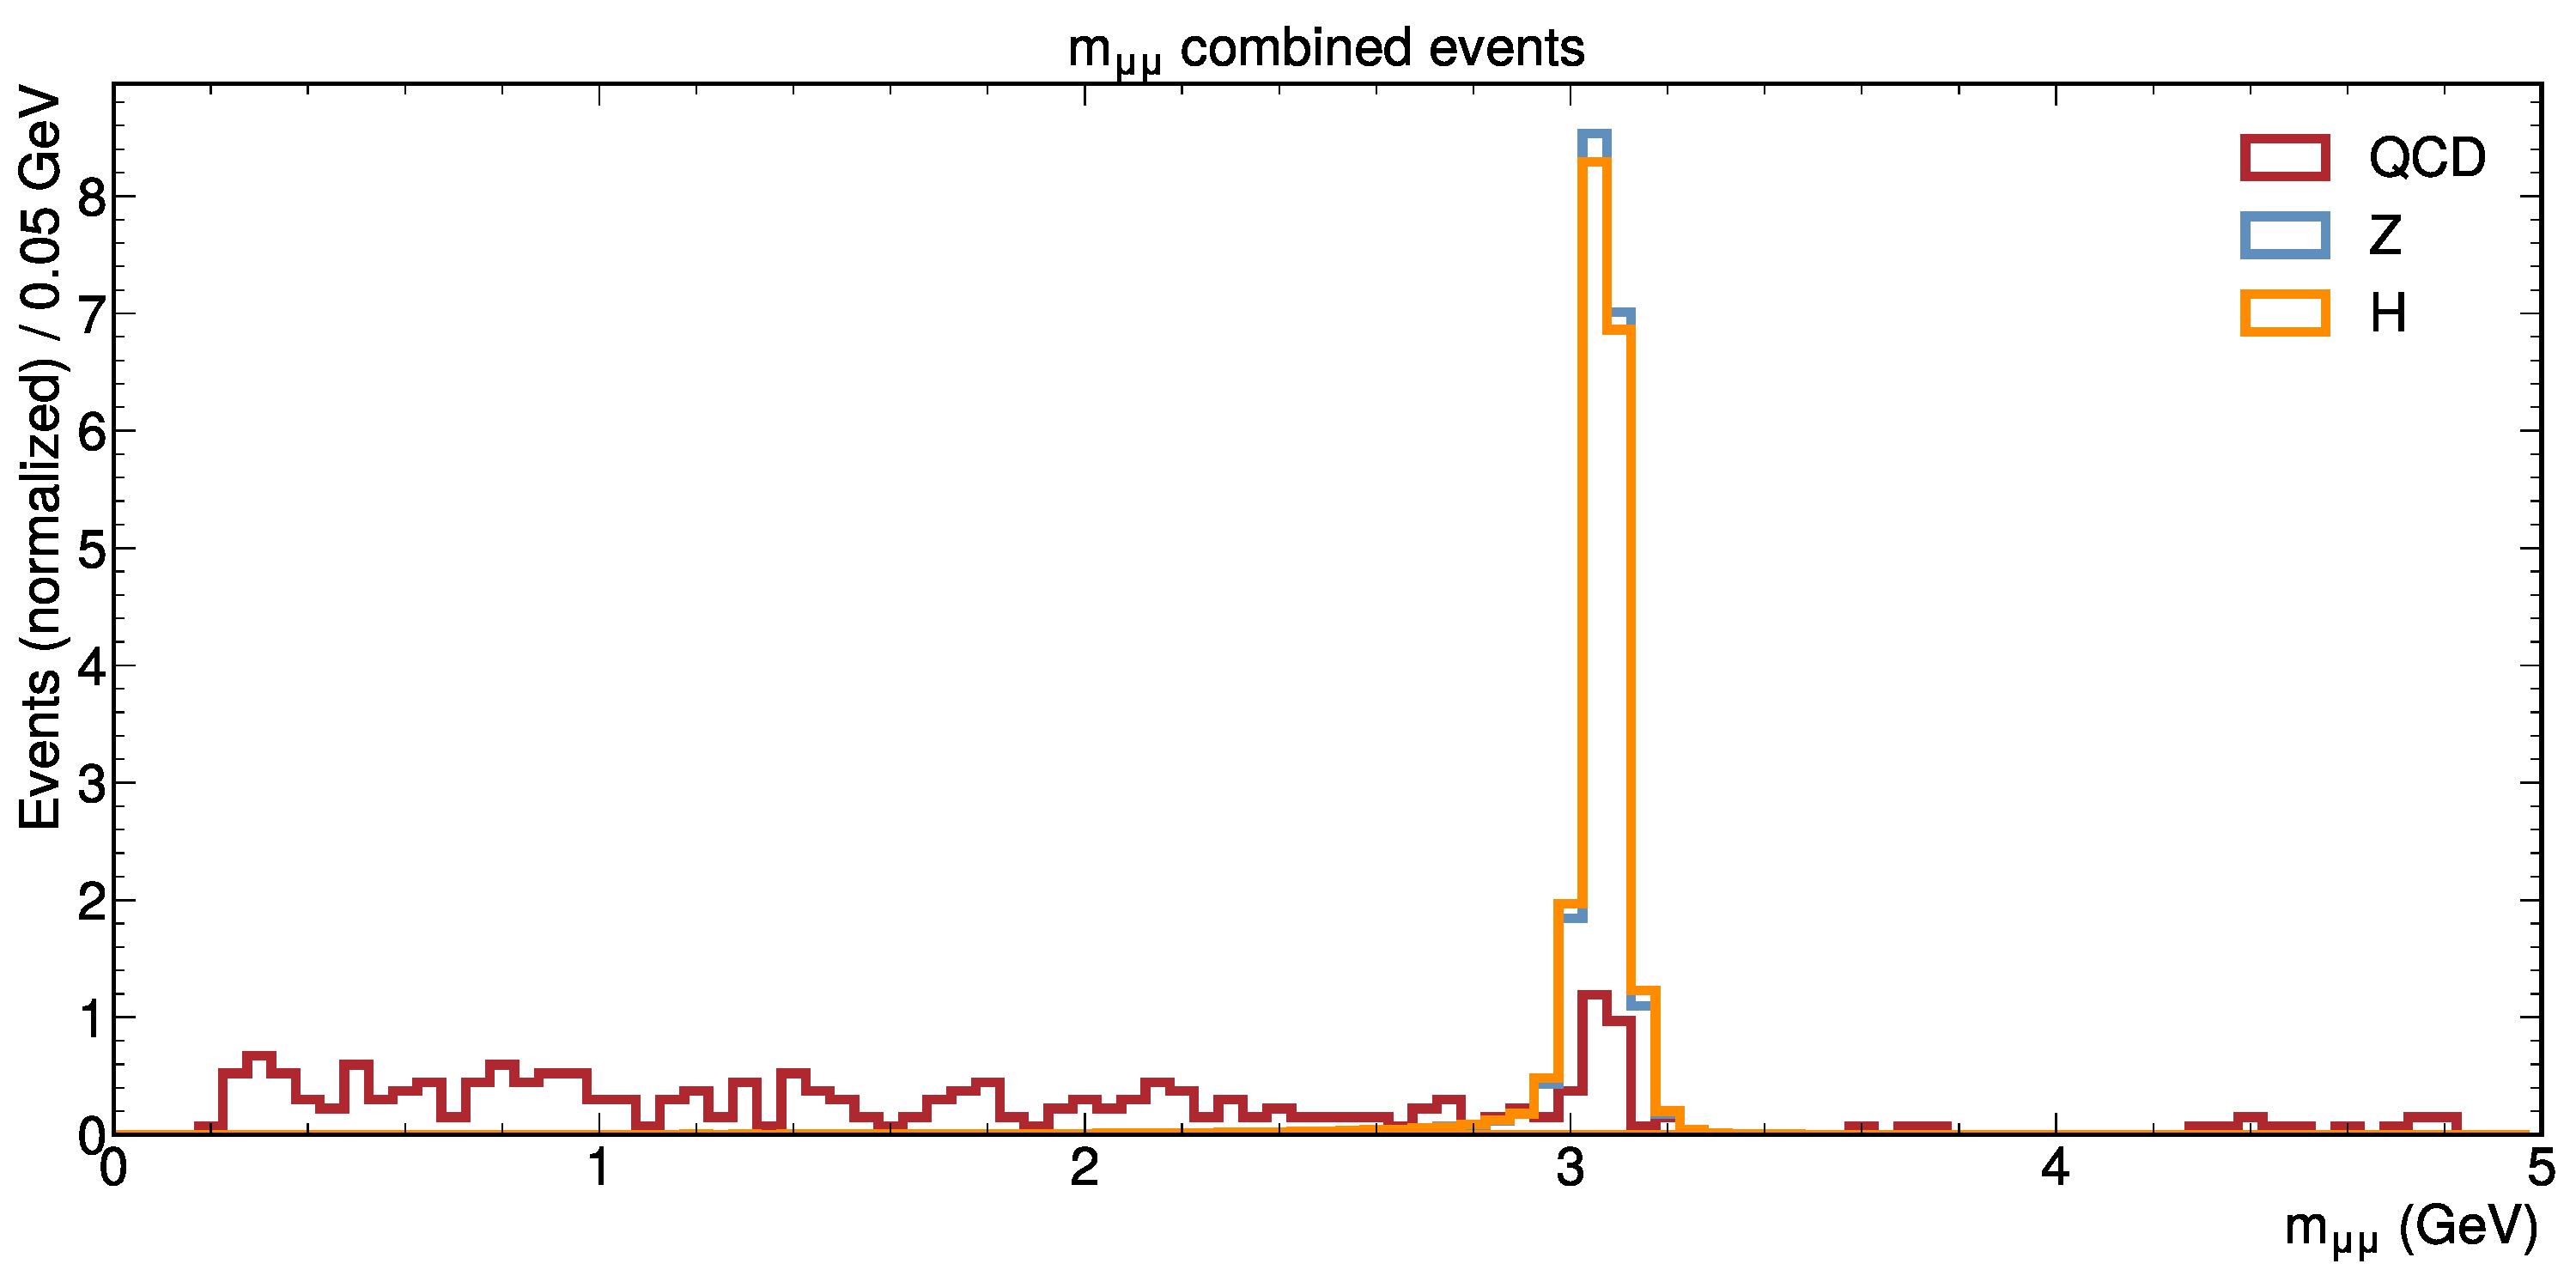
\includegraphics[width=.9\linewidth]{images/m_mumu_combined_TestForCut.pdf}
    \caption{Invariant mass of the muon pair system reconstructed in the final state. Base selection criteria from Table \ref{tab:selection} have been applied in order to observe the distribution in $m_{\mu\mu}$. The number of events in each histogram has been normalized so that the integral is equal to 1.
    \label{im:m_mumu_combined_TestForCut}}
\end{figure}

Similarly to the $\Delta R$ histogram, also in Fig. \ref{im:m_mumu_combined_TestForCut} the QCD events are rather uniform, whereas the Z and Higgs events reconstructed show an accumulation at around 3 GeV.

This is the motivation to have introduced a mass interval selection for the muon pair invariant mass, it being $(2,\ 4)\GeV$. Also, the muon and photon momenta thresholds have been updated to 15 GeV and 20 GeV, respectively. The selection efficiencies obtained for this set of selections are shown in Table \ref{tab:Mu15_Ph20_2mumuM4}.

% Table generated by Excel2LaTeX from sheet 'Tables to present'
\begin{table}[htbp]
  \centering
    \resizebox{\textwidth}{!}{
    \begin{tabular}{ccc}
        \toprule
        & \multicolumn{2}{|c}{Selection efficiencies (\%)} \\ \midrule
        & \multicolumn{1}{|c|}{$\pt^{\mu 1} > 18\GeV$, $\pt^{\gamma} > 32\GeV$} & $\pt^{\mu 1} > 15\GeV$, $\pt^{\gamma} > 20\GeV$, $2 < m_{\mu\mu} < 4\GeV$ \\ \midrule
        QCD   & \multicolumn{1}{|c|}{$(1.6\pm 0.3)\cdot 10^{-4}$} & $(1.3\pm0.2)\cdot 10^{-4}$ \\
        Z     & \multicolumn{1}{|c|}{$21.49\pm0.06$} &  $27.42\pm0.07$ \\
        H     & \multicolumn{1}{|c|}{$35.85\pm 0.07$} &  $38.75\pm0.07$ \\ \bottomrule
    \end{tabular}}
    \caption{Selection efficiencies obtained for the selection cuts: $\pt^{\mu 1} > 15\GeV$, $\pt^{\gamma} > 20\GeV$, $2 <m_{\mu\mu} <4\GeV$ (right column) compared to the ones obtained for $\pt^{\mu 1} > 18\GeV$, $\pt^{\gamma} > 32\GeV$ (left column).
    \label{tab:Mu15_Ph20_2mumuM4}}
\end{table}%

The efficiencies obtained are higher for Z and Higgs signal and lower for QCD, with respect to the ones obtained in Section \ref{sec:Mu18_Ph24_dR04}. Changing the $\Delta R$ cut for that of the muon pair invariant mass, even if using less strict criteria for the muon and the photon momentum thresholds, provides results that are substantially better.

\subsection{Muon1: $\pt > 10\GeV$, muon2: $\pt > 5\GeV$, photon: $\pt>15\GeV$, $2\GeV<m_{\mu\mu}<4\GeV$}
After some iterations, it has been found that one of the optimal configurations of the trigger is one that uses cuts in the momentum of the three particles in the final state i.e. both muons and the photon, while also applying an interval selection for the invariant mass of the muons.

In this subsection, the goal was to find the maximum efficiency reachable for the Z and the Higgs signal, and observe how much the QCD efficiency would increase over the $(1.6\pm0.3)\cdot 10^{-4}$ \% value of {\it HLT\_Mu17\_Photon30}. To do this, the cuts on both muons and photon have been set back to the pre-selected values from Table \ref{tab:selection}. The corresponding obtained efficiencies are shown in Table \ref{tab:Mu10_Mu05_Photon15_2mumuM4}.

% Table generated by Excel2LaTeX from sheet 'Tables to present'
\begin{table}[htbp]
  \centering
    \resizebox{\textwidth}{!}{
    \begin{tabular}{ccc}
        \toprule
        & \multicolumn{2}{|c}{Selection efficiencies (\%)} \\ \midrule
        & \multicolumn{1}{|c|}{$\pt^{\mu 1} > 18\GeV$, $\pt^{\gamma} > 32\GeV$} & $\pt^{\mu 1} > 10\GeV$, $\pt^{\mu 2} > 5\GeV$,\\
        & \multicolumn{1}{|c|}{} & $\pt^{\gamma} > 15\GeV$, $2\GeV < m_{\mu\mu} < 4\GeV$ \\ \midrule
        QCD   & \multicolumn{1}{|c|}{$(1.6\pm 0.3)\cdot 10^{-4}$} & $(4.5\pm0.5)\cdot 10^{-4}$ \\
        Z     & \multicolumn{1}{|c|}{$21.49\pm0.06$} &  $29.83\pm0.07$ \\
        H     & \multicolumn{1}{|c|}{$35.85\pm 0.07$} &  $39.81\pm0.07$ \\ \bottomrule
    \end{tabular}}
    \caption{Selection efficiencies obtained for the selection cuts: $\pt^{\mu 1} > 10\GeV$, $\pt^{\mu 2} > 5\GeV$, $\pt^{\gamma} > 15\GeV$, $2\GeV < m_{\mu\mu} < 4\GeV$ (right column) compared to the ones obtained for $\pt^{\mu 1} > 18\GeV$, $\pt^{\gamma} > 32\GeV$ (left column).
    \label{tab:Mu10_Mu05_Photon15_2mumuM4}}
\end{table}%

As it can be seen from Table \ref{tab:Mu10_Mu05_Photon15_2mumuM4}, the increased efficiency for QCD is of the order of the 181\%, while the increase in the Z boson and Higgs boson signals is around 38\% and 11\%, respectively.


\subsection{Muon1: $\pt > 10\GeV$, muon2: $\pt > 5\GeV$, photon: $\pt>22.7\GeV$, $2\GeV<m_{\mu\mu}<4\GeV$}

After the results from the previous section, an algorithm was developed to try and obtain the best efficiencies for the Z and Higgs signals, while maintaining the QCD as close as possible to the original $(1.6\pm 0.3)\cdot 10^{-4}$ \% value or even decreasing it. The final selection cuts have been determined to be $\pt > 10\GeV$ for the leading muon, $\pt > 5\GeV$ for the subleading muon, $\pt>22.7\GeV$ for the photon, and $2\GeV<m_{\mu\mu}<4\GeV$ for the interval in which the muon pair invariant mass must be comprehended. The corresponding efficiencies for these cuts are shown in Table \ref{tab:Mu10_Mu05_Photon22.7_2mumuM4}.

% Table generated by Excel2LaTeX from sheet 'Tables to present'
\begin{table}[htbp]
  \centering
    \resizebox{\textwidth}{!}{
    \begin{tabular}{ccc}
        \toprule
        & \multicolumn{2}{|c}{Selection efficiencies (\%)} \\ \midrule
        & \multicolumn{1}{|c|}{$\pt^{\mu 1} > 18\GeV$, $\pt^{\gamma} > 32\GeV$} & $\pt^{\mu 1} > 10\GeV$, $\pt^{\mu 2} > 5\GeV$,\\
        & \multicolumn{1}{|c|}{} & $\pt^{\gamma} > 22.7\GeV$, $2\GeV < m_{\mu\mu} < 4\GeV$ \\ \midrule
        QCD   & \multicolumn{1}{|c|}{$(1.6\pm 0.3)\cdot 10^{-4}$} & $(1.6\pm 0.3)\cdot 10^{-4}$ \\
        Z     & \multicolumn{1}{|c|}{$21.49\pm0.06$} &  $28.22\pm0.07$ \\
        H     & \multicolumn{1}{|c|}{$35.85\pm 0.07$} &  $38.90\pm0.07$ \\ \bottomrule
    \end{tabular}}
    \caption{Selection efficiencies obtained for the selection cuts: $\pt^{\mu 1} > 10\GeV$, $\pt^{\mu 2} > 5\GeV$, $\pt^{\gamma} > 22.7\GeV$, $2\GeV < m_{\mu\mu} < 4\GeV$ (right column) compared to the ones obtained for $\pt^{\mu 1} > 18\GeV$, $\pt^{\gamma} > 32\GeV$ (left column).
    \label{tab:Mu10_Mu05_Photon22.7_2mumuM4}}
\end{table}%

For an increase of only around the 3\% in the QCD efficiency, the Z and Higgs signals have been enhanced by 31\% and 9\%, respectively.

\subsection{Summary of results}

The comparison between the efficiencies for {\it HLT\_Mu17\_Photon30}, corresponding to the selection criteria $\pt^{\mu 1} > 18\GeV$, $\pt^{\gamma} > 32\GeV$ (in the left-most part) and the other selection cuts that have been detailed up to now, are shown in Fig. \ref{im:eff_comparison}.

\begin{figure}[htbp]
    \centering
    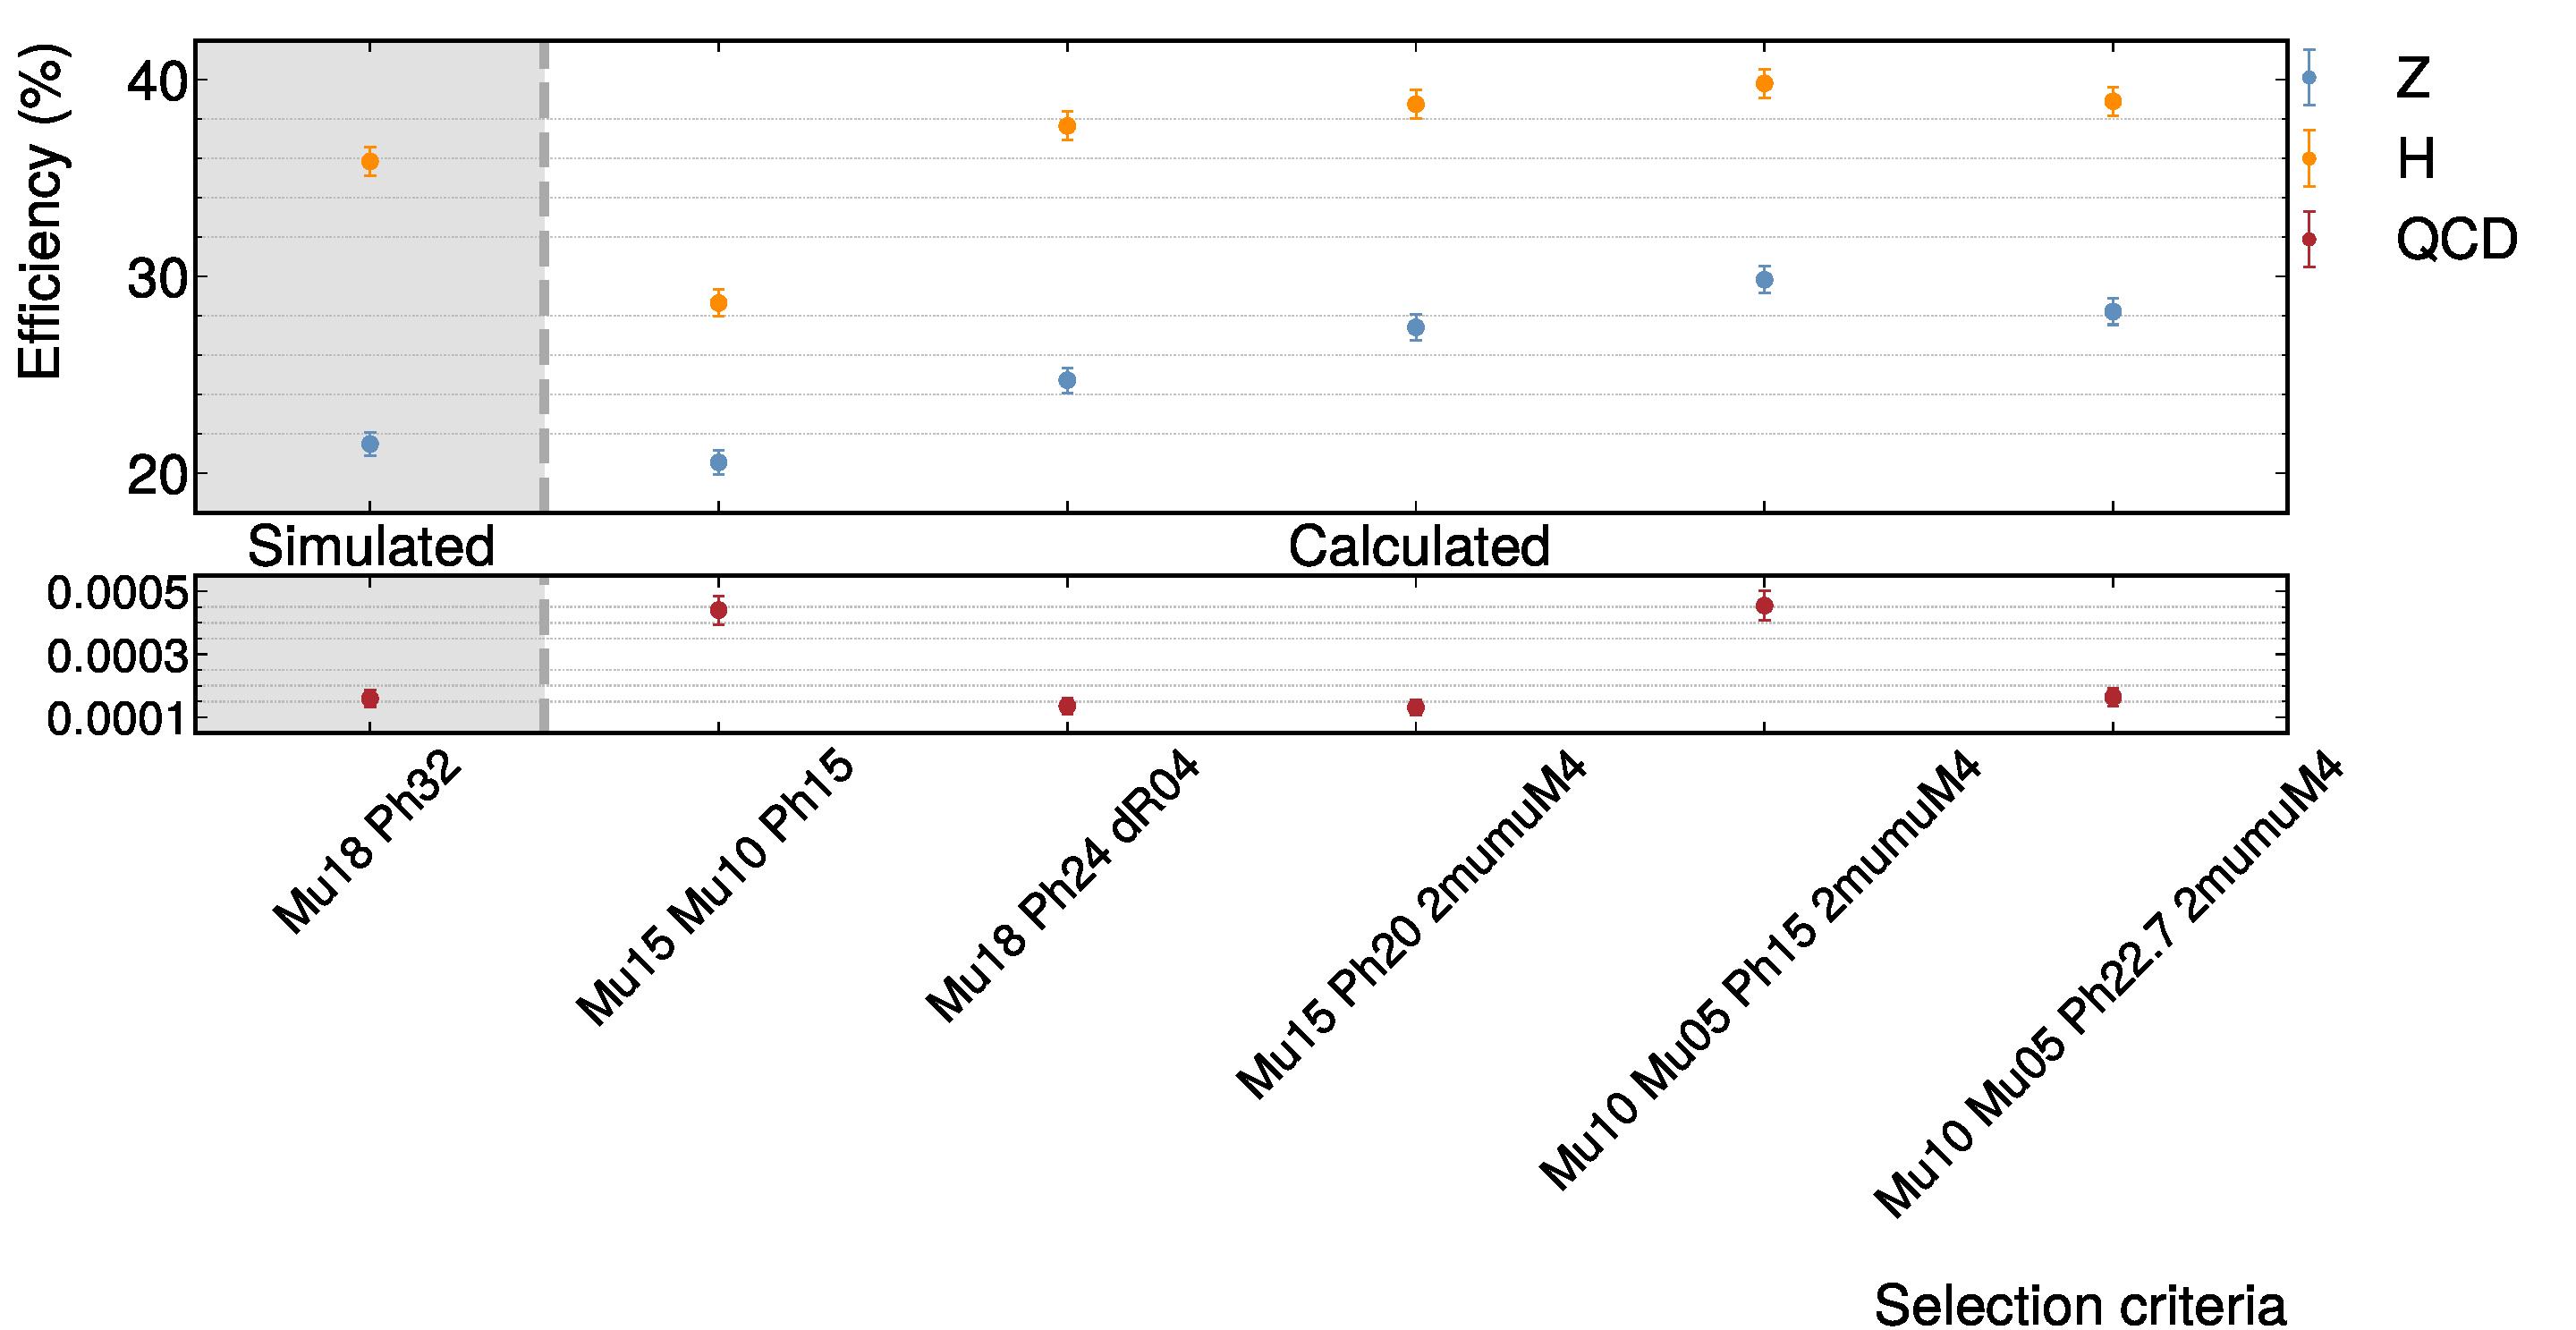
\includegraphics[width=1\linewidth]{images/eff_comparison.pdf}
    \caption{Global display of the selection efficiencies for the different cuts discussed in this section, compared to the ones obtained from {\it HLT\_Mu17\_Photon30} ($\pt^{\mu 1} > 18\GeV$, $\pt^{\gamma} > 32\GeV$), in the left-most part of the graph. Labels of the kind MuX or PhX signify a threshold in the transverse momenta of X GeV, while labels like dR04 and 2mumuM4 are to indicate a selection $\Delta R < 0.4$ and $2\GeV < m_{\mu\mu} < 4\GeV$, respectively.
    \label{im:eff_comparison}}
\end{figure}

As it can be seen, the first filter tested produced a worsening in both signals efficiencies, while enhancing the background, which is the contrary to what is desired.

For the next three filters, increasing efficiencies for the signals have been obtained, while the QCD efficiencies have been around the reference value, or substantially increased in the ``Mu10 Mu05 Ph15 2mumuM4'' case.

In the end, a compromise betweeen both type of efficiencies is believed to be achieved with the selection cuts: $\pt^{\mu 1} > 10\GeV$, $\pt^{\mu 2} > 5\GeV$, $\pt^{\gamma} > 22.7\GeV$, $2\GeV < m_{\mu\mu} < 4\GeV$. Rising the momentum threshold in photons from $15\GeV$ to $22.7\GeV$ causes a slight decrease in the signals efficiencies, but reduces the QCD efficiency drastically.

\section{Conclusions}

A study of the efficiency of the trigger {\it HLT\_Mu17\_Photon30} has been presented. This trigger is currently used in the study of the exotic Higgs boson decay $\H \rightarrow \JPsi\gamma \rightarrow \mu\mu\gamma$, for which the analogue Z boson decay is used as an experimental benchmark. As explained in Section \ref{sec:introduction}, the low signal-to-background ratio of these reactions turn the selection and trigger efficiencies into a critical experimental aspect.

In order to obtain the selection efficiencies for every set of criteria, the number of events passing the selection have been divided by the total number of events generated by the Monte Carlo. Then, these values have been compared to the standard selection $\pt^{\mu 1}>18\GeV$ and $\pt^{\gamma}>32\GeV$, corresponding to the {\it HLT\_Mu17\_Photon30} implemented trigger. The interplay between background and signal efficiencies imposes a finite range of parameters to be used, which have to be finely tuned in order to minimize the former and maximize the latter.

As a result, it has been found that different types of criteria, besides those purely kinematical, should be used in order to obtain optimal efficiencies. In particular, the selection in muons angular separation and, more importantly, the selection in muons pair invariant mass, have proven to be more adequate for the discrimination of signal and background.

All in all, it must be reminded that the selection efficiencies calculated are not trigger efficiencies (i.e. the fraction of events that pass the logical trigger within a given selection); dedicated simulations are needed to estimate those. However, this work hints at other types of triggers that are feasible and could outperform the current ones in terms of efficiency. In order to determine this more precisely, future studies on the topic will be needed.

%%%%%%%Bibliografía
\appendix
\cleardoublepage
\bibliography{bibliography.bib}
\end{document}